\documentclass[border=8pt, multi, tikz]{standalone}
\usepackage{import}
\usepackage{graphicx}
\usetikzlibrary{shapes, arrows}
\subimport{../layers/}{init}

\newcommand\DrawDiagonal[4][1]{
	\foreach \s in {0,1,...,#4}
	{
		\node [minimum size = 1cm, fill=red, opacity=#1] at (#2+\s+0.5,#3-\s-0.5){};
	}
}
\newcommand*{\xMin}{-28}
\newcommand*{\yMin}{-28}
\newcommand*{\xMax}{29}
\newcommand*{\yMax}{29}

\begin{document}
	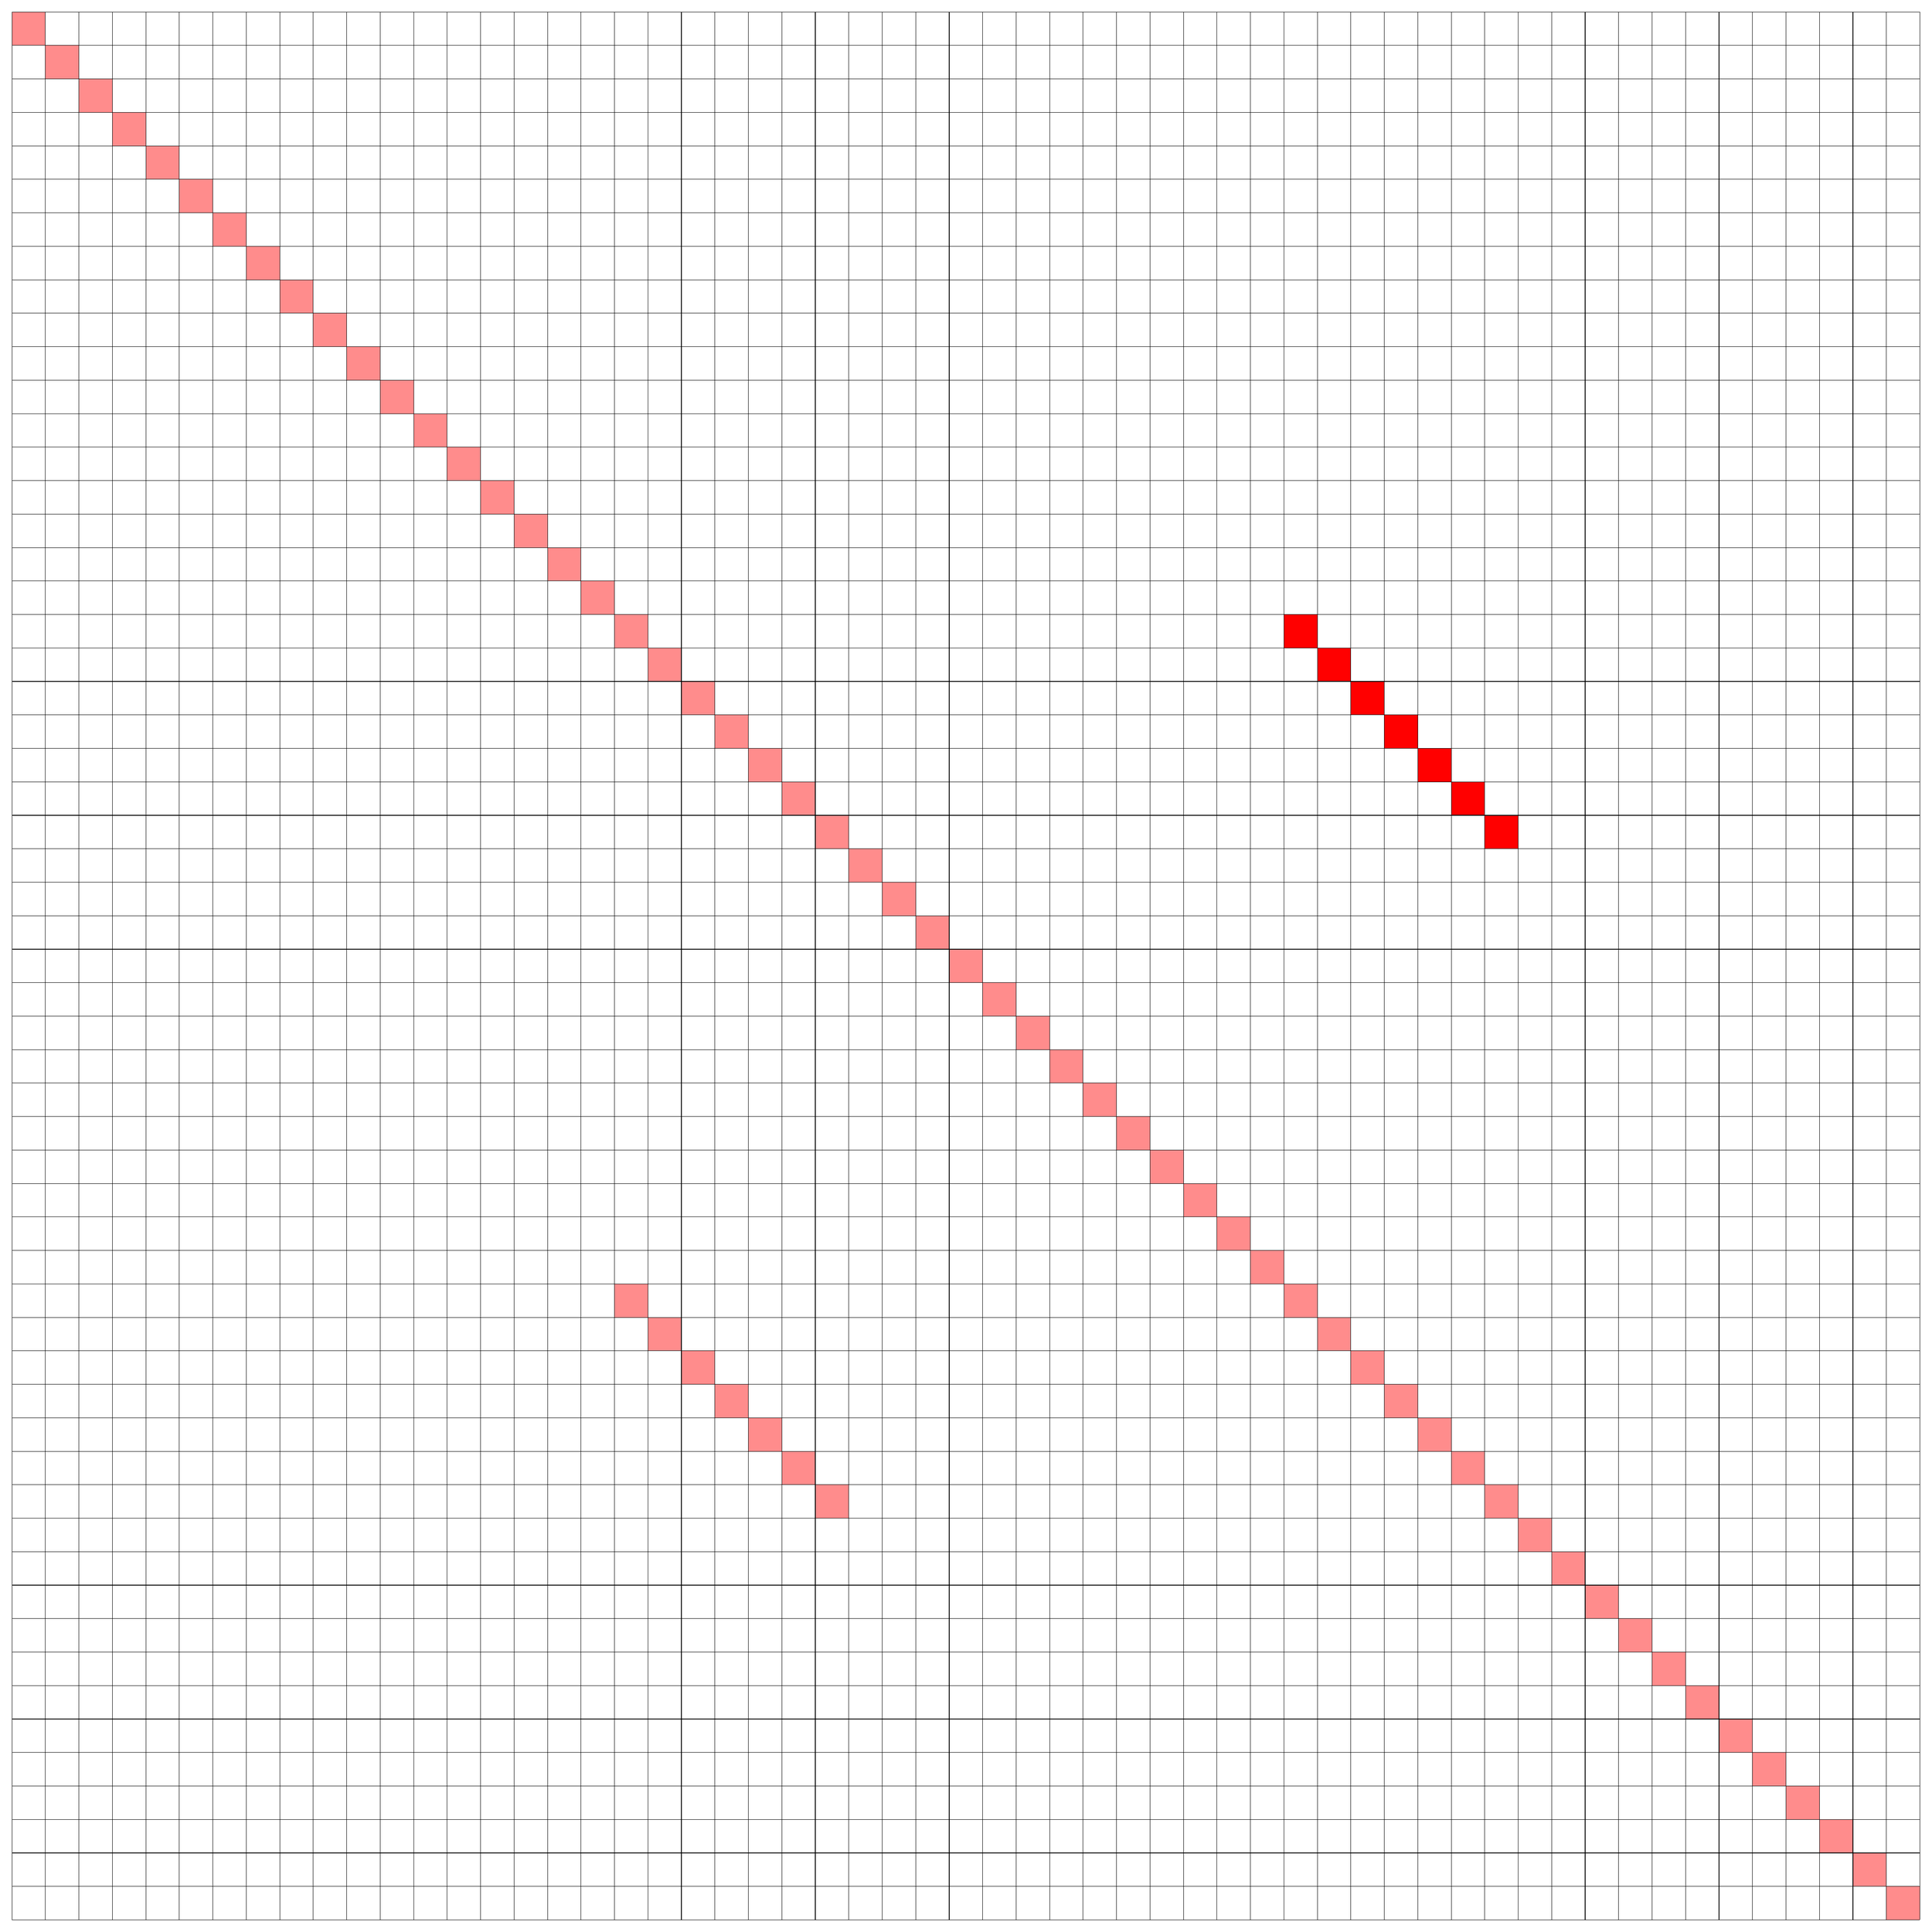
\begin{tikzpicture}[every node/.style={minimum size=1cm-\pgflinewidth, outer sep=0pt, fill=green}]
%	\foreach \x in {-25,-24,...,24}
%	{
%		\node [opacity=0.5, minimum size = 1cm] at (\x+0.5,-\x-0.5){};
%	}
%	\foreach \x in {-24,-23,...,24}
%	{
%		\node [minimum size = 1cm] at (\x+0.5,-\x+0.5){};
%		\node [minimum size = 1cm] at (\x-0.5,-\x-0.5){};
%	}
%	\DrawDiagonal{-8}{20}{10}
%	\DrawDiagonal{6}{6}{5}
%	\DrawDiagonal{-20}{-8}{9}
	\DrawDiagonal{10}{11}{6}
	\DrawDiagonal[0.45]{-10}{-9}{6}
	\DrawDiagonal[0.45]{\xMin}{\yMax}{56}
%	\path [draw, line width=5pt, ->, >=Triangle] (-19.5,-8.5) -- (-19.5, \yMax);
%	\path [draw, line width=5pt, ->, >=Triangle] (-19.5,-8.5) -- (\xMin, -8.5);
%	\path [draw, line width=5pt, ->, >=Triangle] (-10.5,-17.5) -- (-10.5, \yMax);
%	\path [draw, line width=5pt, ->, >=Triangle] (-10.5,-17.5) -- (\xMin, -17.5);
%	\DrawDiagonal{\xMin}{\yMax}{\xMax+\yMax}
%	\node [fill=black] at (0.5,-0.5) {};
%	\node[rectangle, minimum size=5cm, fill=black] at (\xMin,\yMax);
% vertical
%	\node[shift={(0,0)}, above left, rotate=90, inner sep=0] (waveform_1) at (\xMin,\yMax) 	{\includegraphics[width=\linewidth]{../examples/sample_sentence.png}};
%	
%	\node[shift={(0,0)}, left, rotate=90, inner sep=0] (waveform_2) at (waveform_1) 	{\includegraphics[width=\linewidth]{../examples/sample_sentence.png}};
%	
%	\node [draw, rectangle, rotate=90, fill=lightgray, left, minimum height = 151pt, minimum width =0.6\linewidth] (yes) at (waveform_2.west) {{\Huge\bfseries yes}};
%
%	\node[shift={(0,-0.15)}, left, rotate=90, inner sep=0] (waveform_3) at (yes.west) 	{\includegraphics[width=\linewidth]{../examples/sample_sentence.png}};
%	
%	\node [draw, rectangle, rotate=90, fill=lightgray, left, minimum height = 151pt, minimum width =0.6\linewidth] (yes_2) at (waveform_3.west) {{\Huge\bfseries yes}};
%
%	\node[shift={(0,-0.15)}, left, rotate=90, inner sep=0] (waveform_2) at (yes_2.west) 	{\scalebox{-1}[1]{\includegraphics[width=\linewidth]{../examples/sample_sentence.png}}};		
	
% horizontal	
%	\node[shift={(0,0)}, above right, inner sep=0] (waveform_3) at (\xMin,\yMax) {\includegraphics[width=\linewidth]{../examples/sample_sentence.png}};
%	
%	\node[shift={(0,0)}, right, inner sep=0] (waveform_4) at (waveform_3) 	{\includegraphics[width=\linewidth]{../examples/sample_sentence.png}};
%	
%	\node [draw, rectangle, fill=lightgray, right, minimum height = 151pt, minimum width =0.6\linewidth] (yes) at (waveform_4.east) {{\Huge\bfseries yes}};
%	
%	\node[shift={(0.2,0)}, right, inner sep=0] (waveform_4) at (yes.east) 	{\includegraphics[width=\linewidth]{../examples/sample_sentence.png}};
%	
%	\node [draw, rectangle, fill=lightgray, right, minimum height = 151pt, minimum width =0.6\linewidth] (no) at (waveform_4.east) {{\Huge\bfseries no}};
%	
%	\node[shift={(0.2,0)}, right, inner sep=0] (waveform_4) at (no.east) 	{\scalebox{-1}[1]{\includegraphics[width=\linewidth]{../examples/sample_sentence.png}}};
	
	\draw[step=1cm,color=black](\xMin,\yMin) grid (\xMax, \yMax);
	\end{tikzpicture}
\end{document}